\documentclass[11pt]{article}

% PACKAGES
\usepackage{amsmath}
\usepackage{amssymb}
\usepackage{graphicx}
\usepackage[margin=1in]{geometry}
\usepackage{hyperref}
\usepackage{tikz}
\usetikzlibrary{arrows.meta}

% DOCUMENT INFO
\title{New Problems in Electromagnetic Induction}
\author{}
\date{\today}

\begin{document}

\maketitle
\tableofcontents
\newpage

\section{New Problem 1: Rod Sliding on an Inclined Plane}
This problem combines motional EMF with mechanics, similar to the setup in `EMI3.pdf` but adding the element of gravity.

\subsection{Question}
A conducting rod of mass $m = 50 \text{ g}$ and resistance $R = 0.25 \, \Omega$ is placed on two frictionless, parallel conducting rails inclined at an angle $\theta = 30^\circ$ to the horizontal. The rails have negligible resistance and are connected at the bottom by a wire. The entire setup is in a uniform vertical magnetic field of magnitude $B = 0.50 \text{ T}$, as shown in the diagram. The rod is released from rest.

\begin{center}
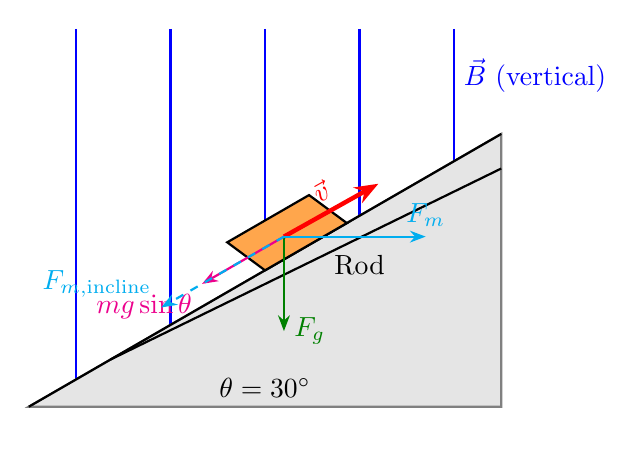
\begin{tikzpicture}[scale=1.2, rotate=0]
    % Draw B field vectors (vertical)
    \foreach \x in {0.5, 1.5, 2.5, 3.5, 4.5} {
        \draw[-{Stealth[length=2mm]}, thick, blue] (\x, 4) -- (\x, 0) node[below] {};
    }
    \node[blue, right] at (4.5, 3.5) {$\vec{B}$ (vertical)};
    
    % Draw inclined plane
    \draw[thick, gray, fill=gray!20] (0,0) -- (5,0) -- (5, 2.887) -- cycle; % 5*tan(30) = 2.887
    
    % Draw rails on the incline
    \draw[thick] (0.866, 0.5) -- (5, 2.887 - 0.5*1.732 + 0.5); % Rail 1
    \draw[thick] (0,0) -- (5, 2.887); % Rail 2
    \node at (2.5, 0.2) {$\theta=30^\circ$};
    
    % Draw conducting rod
    \draw[thick, fill=orange!70] (2.5, 1.4435) -- (3.366, 1.9435) -- (2.966, 2.24) -- (2.1, 1.74) -- cycle;
    \node at (3.5, 1.5) {Rod};
    
    % Velocity vector
    \draw[-{Stealth[length=3mm]}, ultra thick, red] (2.7, 1.8) -- (3.7, 2.36) node[midway, above, sloped] {$\vec{v}$};
    
    % Force vectors on the rod (as a point for clarity)
    \coordinate (rodcenter) at (2.7, 1.8);
    \draw[-{Stealth[length=2mm]}, thick, green!50!black] (rodcenter) --++ (0,-1) node[right]{$F_g$};
    \draw[-{Stealth[length=2mm]}, thick, magenta] (rodcenter) --++ (-1.732/2, -1/2) node[below left]{$mg\sin\theta$};
    \draw[-{Stealth[length=2mm]}, thick, cyan] (rodcenter) --++ (1.5,0) node[above]{$F_m$};
    \draw[-{Stealth[length=2mm]}, thick, cyan, dashed] (rodcenter) --++ (-1.5*0.866, -1.5*0.5) node[above left]{$F_{m, \text{incline}}$};
\end{tikzpicture}
\end{center}

\begin{enumerate}
    \item[(a)] Find the terminal velocity ($v_t$) of the rod as it slides down the incline.
    \item[(b)] What is the magnitude of the induced current at this terminal velocity?
    \item[(c)] Show that the rate of electrical energy dissipation is equal to the rate of gravitational potential energy loss at terminal velocity.
\end{enumerate}

\subsection{Explanation and Solution}
\begin{enumerate}
    \item[(a)] \textbf{Finding the Terminal Velocity}\\
    The magnetic flux through the loop is $\Phi_B = \vec{B} \cdot \vec{A} = B A \cos\theta$, where $A=Lx$ is the area of the loop and $x$ is the distance the rod has slid.
    The induced EMF is $|\mathcal{E}| = \frac{d\Phi_B}{dt} = \frac{d}{dt}(BLx \cos\theta) = BLv \cos\theta$.
    The induced current is $I = \frac{\mathcal{E}}{R} = \frac{BLv \cos\theta}{R}$.
    The magnetic force on the rod is horizontal with magnitude $F_m = ILB$. Its component opposing motion along the incline is $F_{m, \text{incline}} = F_m \cos\theta = (ILB)\cos\theta$.
    At terminal velocity ($v_t$), the net force is zero, so the gravitational component pulling the rod down is balanced by the magnetic component pushing it up the incline.
    $$ mg \sin\theta = F_{m, \text{incline}} $$
    $$ mg \sin\theta = \left(\frac{BLv_t \cos\theta}{R}\right)LB\cos\theta = \frac{B^2 L^2 v_t \cos^2\theta}{R} $$
    Solving for $v_t$ and assuming a standard rail width $L=1.0 \text{ m}$:
    $$ v_t = \frac{mgR \sin\theta}{B^2 L^2 \cos^2\theta} = \frac{(0.050)(9.8)(0.25)\sin(30^\circ)}{(0.50)^2 (1.0)^2 \cos^2(30^\circ)} = \mathbf{0.327 \, m/s} $$

    \item[(b)] \textbf{Current at Terminal Velocity}\\
    Substitute $v_t$ back into the equation for current:
    $$ I = \frac{BLv_t \cos\theta}{R} = \frac{(0.50)(1.0)(0.327)\cos(30^\circ)}{0.25} = \mathbf{0.566 \, A} $$

    \item[(c)] \textbf{Energy Conservation}\\
    Rate of electrical energy dissipation (power):
    $$ P_{elec} = I^2R = (0.566)^2(0.25) = \mathbf{0.080 \, W} $$
    Rate of gravitational potential energy loss:
    $$ P_{grav} = (mg \sin\theta) v_t = (0.050)(9.8)\sin(30^\circ)(0.327) = \mathbf{0.080 \, W} $$
    Since $P_{elec} = P_{grav}$, energy is conserved.
\end{enumerate}
\hrule

\section{New Problem 2: The Levitating Square Coil}
This problem tests the concept of magnetic force in a non-uniform field.

\subsection{Question}
A square coil with side length $l = 10 \text{ cm}$, $N=50$ turns, and mass $m = 100 \text{ g}$ is positioned in a non-uniform magnetic field. The magnetic field is horizontal but its magnitude increases vertically upwards, given by $\vec{B}(y) = (ky) \hat{x}$, where $k = 2.0 \text{ T/m}$. The coil is in the y-z plane. What is the magnitude and direction of the current $I$ required for the coil to levitate?

\begin{center}
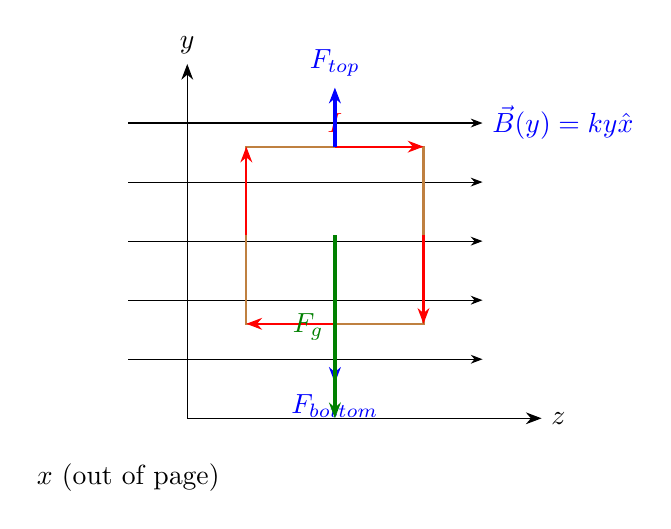
\begin{tikzpicture}[scale=1.5]
    % Y and Z axes
    \draw[-{Stealth[length=2mm]}] (0,0) -- (0,3) node[above] {$y$};
    \draw[-{Stealth[length=2mm]}] (0,0) -- (3,0) node[right] {$z$};
    \node at (-0.5,-0.5) {$x$ (out of page)};

    % Magnetic field lines (horizontal, increasing density upwards)
    \foreach \y in {0.5, 1, 1.5, 2, 2.5} {
        \draw[-{Stealth[length=1.5mm]}] (-0.5, \y) -- (2.5, \y);
    }
    \node[blue, right] at (2.5, 2.5) {$\vec{B}(y) = ky\hat{x}$};

    % Square coil
    \draw[thick, brown] (0.5, 0.8) rectangle (2, 2.3);
    
    % Current direction arrows
    \draw[-{Stealth[length=2mm]}, red, thick] (0.5, 1.55) -- (0.5, 2.3); % Left side up
    \draw[-{Stealth[length=2mm]}, red, thick] (1.25, 2.3) -- (2, 2.3); % Top side right (+z)
    \draw[-{Stealth[length=2mm]}, red, thick] (2, 1.55) -- (2, 0.8); % Right side down
    \draw[-{Stealth[length=2mm]}, red, thick] (1.25, 0.8) -- (0.5, 0.8); % Bottom side left (-z)
    \node[red] at (1.25, 2.5) {$I$};
    
    % Force vectors
    \draw[-{Stealth[length=2mm]}, ultra thick, blue] (1.25, 0.8) -- (1.25, 0.3) node[below] {$F_{bottom}$};
    \draw[-{Stealth[length=2mm]}, ultra thick, blue] (1.25, 2.3) -- (1.25, 2.8) node[above] {$F_{top}$};
    \draw[-{Stealth[length=2mm]}, ultra thick, green!50!black] (1.25, 1.55) -- (1.25, 0) node[midway, left] {$F_g$};
\end{tikzpicture}
\end{center}

\subsection{Explanation and Solution}
The forces on the vertical sides of the coil are in the $\pm \hat{z}$ direction and cancel each other out. We only need to consider the horizontal sides.
\begin{itemize}
    \item \textbf{Bottom Side (at y):} The force is downwards. $\vec{F}_{bottom} = I (l(-\hat{z})) \times (ky \hat{x}) = -Ikly \hat{y}$.
    \item \textbf{Top Side (at y+l):} The force is upwards. $\vec{F}_{top} = I (l(\hat{z})) \times (k(y+l) \hat{x}) = Ikl(y+l) \hat{y}$.
\end{itemize}
The net magnetic force for $N$ turns is:
$$ \vec{F}_{net, m} = N(\vec{F}_{top} + \vec{F}_{bottom}) = N(Ikl(y+l) - Ikly)\hat{y} = NIkl^2 \hat{y} $$
For levitation, this must balance gravity ($F_g = mg$):
$$ NIkl^2 = mg $$
Solving for the current $I$:
$$ I = \frac{mg}{Nkl^2} = \frac{(0.100 \text{ kg})(9.8 \text{ m/s}^2)}{(50)(2.0 \text{ T/m})(0.10 \text{ m})^2} = \mathbf{0.98 \, A} $$
The direction must be as shown in the diagram to produce an upward force on the top wire.

\hrule

\section{New Problem 3: The Faraday Disk}
This problem explores motional EMF in a solid rotating disk.

\subsection{Question}
A copper disk of radius $a = 20 \text{ cm}$ rotates at $\omega = 300 \text{ rad/s}$ in a uniform magnetic field $B = 1.5 \text{ T}$ perpendicular to its plane. A circuit is formed using sliding contacts at the center and the rim, connected to a resistor $R_0 = 2.0 \, \Omega$. The disk's resistance is negligible.

\begin{center}
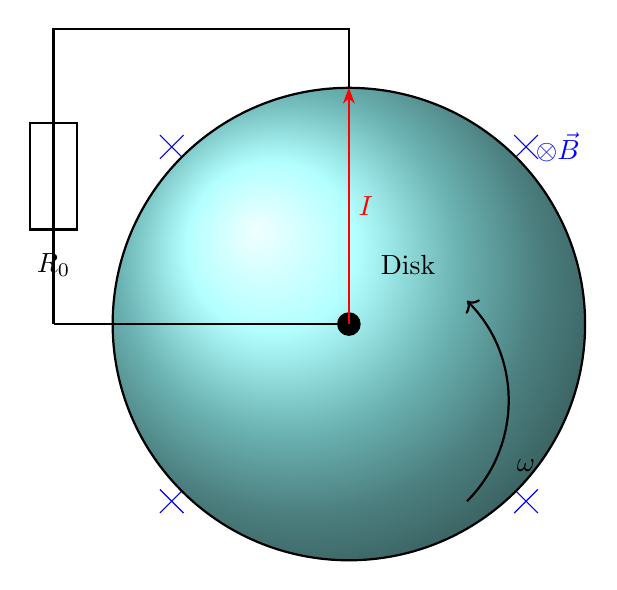
\begin{tikzpicture}[scale=1.5]
    % B-field (into page)
    \foreach \x in {-1.5, -0.5, 0.5, 1.5}
        \foreach \y in {-1.5, -0.5, 0.5, 1.5} {
            \draw[blue] (\x-0.1, \y-0.1) -- (\x+0.1, \y+0.1);
            \draw[blue] (\x-0.1, \y+0.1) -- (\x+0.1, \y-0.1);
        }
    \node[blue, right] at (1.5, 1.5) {$\otimes \vec{B}$};

    % Disk
    \shade[ball color=cyan!40] (0,0) circle (2cm);
    \draw[thick] (0,0) circle (2cm);
    \fill (0,0) circle (0.1cm);
    \node at (0.5, 0.5) {Disk};
    
    % Rotation
    \draw[->, thick] (1, -1.5) arc (-45:45:1.2cm);
    \node at (1.5, -1.2) {$\omega$};
    
    % External circuit
    \draw[thick] (0,0) -- (-2.5, 0); % Axle contact
    \draw[thick] (0, 2) -- (0, 2.5) -- (-2.5, 2.5) -- (-2.5, 0); % Rim contact
    \draw[thick] (-2.7, 0.8) rectangle (-2.3, 1.7); % Resistor
    \node at (-2.5, 0.5) {$R_0$};
    
    % Current flow
    \draw[-{Stealth[length=2mm]}, red, thick] (0,0) -- (0,2);
    \node[red, right] at (0,1) {$I$};
\end{tikzpicture}
\end{center}

\begin{enumerate}
    \item[(a)] What is the magnitude of the EMF induced between the center and the rim?
    \item[(b)] What is the current that flows through the external resistor?
    \item[(c)] Calculate the external torque required to keep the disk rotating.
\end{enumerate}

\subsection{Explanation and Solution}
\begin{enumerate}
    \item[(a)] \textbf{Induced EMF}\\
    We integrate the motional EMF $d\mathcal{E} = Bv\,dr = B(\omega r)dr$ from the center to the rim.
    $$ \mathcal{E} = \int_{0}^{a} B\omega r \, dr = B\omega \left[ \frac{r^2}{2} \right]_{0}^{a} = \frac{1}{2} B\omega a^2 $$
    $$ \mathcal{E} = \frac{1}{2} (1.5)(300)(0.20)^2 = \mathbf{9.0 \, V} $$
    
    \item[(b)] \textbf{Current}\\
    Using Ohm's law with the external resistor:
    $$ I = \frac{\mathcal{E}}{R_0} = \frac{9.0 \text{ V}}{2.0 \, \Omega} = \mathbf{4.5 \, A} $$
    
    \item[(c)] \textbf{External Torque}\\
    The current $I$ flowing radially in the magnetic field creates a drag torque. We integrate the torque element $d\tau_m = r \, dF_m = r(IB\,dr)$ from center to rim.
    $$ \tau_m = \int_{0}^{a} rIB \, dr = IB \left[ \frac{r^2}{2} \right]_{0}^{a} = \frac{1}{2} I B a^2 $$
    The external torque must balance this drag torque:
    $$ \tau_{ext} = \frac{1}{2} (4.5 \text{ A})(1.5 \text{ T})(0.20 \text{ m})^2 = \mathbf{0.135 \, N \cdot m} $$
\end{enumerate}
\hrule

\section{New Problem 4: The Expanding Loop}
This problem involves a changing loop area and the application of Faraday's Law.

\subsection{Question}
A square conducting loop of initial side length $x_0$ and resistance $R$ is being pulled outwards from two opposite sides. Each side moves with a constant velocity $v_0$. The loop remains in a uniform magnetic field $B$ perpendicular to its plane.

\begin{center}
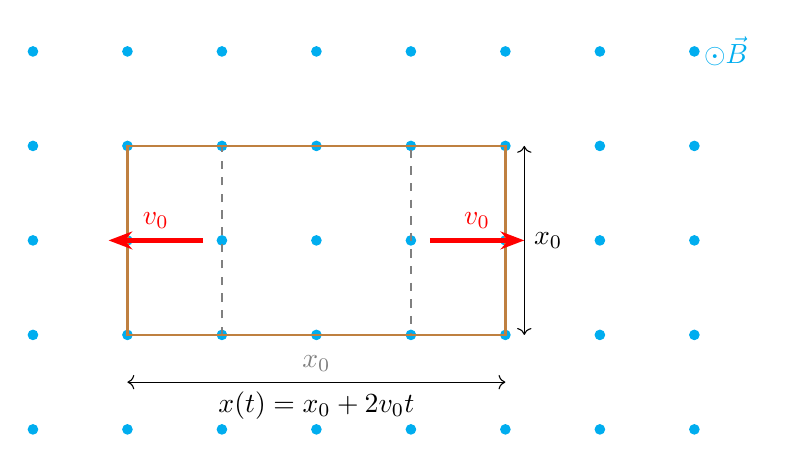
\begin{tikzpicture}[scale=1.2]
    % B-field (dots)
    \foreach \x in {-2,-1,...,5}
        \foreach \y in {-1,...,3}
            \filldraw[cyan] (\x,\y) circle (0.05cm);
    \node[cyan, right] at (5, 3) {$\odot \vec{B}$};

    % Initial loop (dashed)
    \draw[thick, dashed, gray] (0,0) rectangle (2,2);
    \node[gray] at (1,-0.3) {$x_0$};
    
    % Expanding loop at time t
    \draw[thick, brown] (-1,0) rectangle (3,2);
    
    % Velocity vectors
    \draw[-{Stealth[length=3mm]}, ultra thick, red] (-0.2, 1) -- (-1.2, 1) node[midway, above] {$v_0$};
    \draw[-{Stealth[length=3mm]}, ultra thick, red] (2.2, 1) -- (3.2, 1) node[midway, above] {$v_0$};
    
    % Dimensions
    \draw[<->] (-1, -0.5) -- (3, -0.5) node[midway, below] {$x(t) = x_0 + 2v_0t$};
    \draw[<->] (3.2, 0) -- (3.2, 2) node[midway, right] {$x_0$};
\end{tikzpicture}
\end{center}

\begin{enumerate}
    \item[(a)] Find an expression for the induced EMF in the loop as a function of time.
    \item[(b)] Find an expression for the magnitude of the external force required to pull one side of the loop at the constant velocity $v_0$.
\end{enumerate}

\subsection{Explanation and Solution}
\begin{enumerate}
    \item[(a)] \textbf{Induced EMF}\\
    The area of the loop at time $t$ is a rectangle with sides $x_0$ and $(x_0+2v_0t)$.
    $$ A(t) = x_0 (x_0 + 2v_0 t) $$
    The magnetic flux is $\Phi_B = B \cdot A(t) = Bx_0(x_0 + 2v_0 t)$.
    Using Faraday's Law, the magnitude of the EMF is the rate of change of flux:
    $$ |\mathcal{E}| = \left|-\frac{d\Phi_B}{dt}\right| = \left|-\frac{d}{dt} [Bx_0^2 + 2Bx_0v_0 t]\right| $$
    $$ |\mathcal{E}| = 2Bx_0v_0 $$
    The induced EMF is constant.
    
    \item[(b)] \textbf{External Force}\\
    The induced current is $I = \frac{|\mathcal{E}|}{R} = \frac{2Bx_0v_0}{R}$.
    This current flows through the side being pulled (which has length $x_0$), creating a magnetic drag force that opposes the motion.
    $$ F_m = I L B = \left(\frac{2Bx_0v_0}{R}\right) x_0 B = \frac{2B^2x_0^2v_0}{R} $$
    To maintain a constant velocity, the external force must be equal in magnitude to this drag force.
    $$ F_{ext} = \frac{2B^2x_0^2v_0}{R} $$
\end{enumerate}


\end{document}